\section*{Parsing}

In this part we take the token stream and generate an abstract syntax tree (AST). Parsing itself does not check things such as variable scoping, type agreement etc. \medskip

Parsing uses a more powerful tool than regex - context free grammars (CFG). \medskip

Chomsky Hierarchy:
\begin{compactitem}
	\item Regular - Productions have at most one nonterminal and it is at the start or end of the word
	\item Context-Free (CFG) - LHS of productions only have a single nonterminal
	\item Context-Sensitive
	\item Recursively Enumerable
\end{compactitem}

An example for a non CFG would be $a^n b^m c^n d^m$. This corresponds to methods having matching parameters.\medskip

A CFG consists of a set of terminals, a set of nonterminals, a start symbol and a set of productions. A production consists of a single nonterminal LHS and an arbitrary RHS. \medskip

Derivation Orders - Productions can be applied in any order, however they will all lead to the same parse tree. There are two standard orders:
\begin{compactitem}
	\item Leftmost derivation: Find the left-most nonterminal and apply a production to it
	\item Rightmost derivation: Find the right-most nonterminal and apply a production there
\end{compactitem}

A grammar is \textbf{ambiguous} if there are multiple derivation trees for the same word. This can be a problem for associative operators. \medskip

In CFGs ambiguity can (often) be removed by adding nonterminals and allowing recursion only on one side. For example, we want $+$ to be left associative, $*$ right associative and $*$ has the higher precedence:\smallskip

\begin{lstlisting}
	S -> S + S | S * S | (S) | n
\end{lstlisting} \smallskip

Becomes:\smallskip

\begin{lstlisting}
	S_0 -> S_0 + S_1 | S_1
	S_1 -> S_2 * S_1 | S_2
	S_2 -> n | (S_0)
\end{lstlisting}


\subsection*{LL Grammars and Top-Down Parsing}

When parsing a grammar \textbf{top-down}, we can encounter the problem of multiple productions being possible. \medskip

LL(1) means \textbf{L}eft-to-right scanning, \textbf{L}eft-most derivation, \textbf{1} lookahead symbol. \medskip

Left-factoring a grammar can make it LL(1): If there is a common prefix we can add a new non-terminal at the decision point. We also need to eliminate left-recursion:\smallskip

\begin{lstlisting}
 	S -> S a_1 | ... | S a_n | b_1 | ... | b_m
\end{lstlisting}\smallskip

Becomes:\smallskip

\begin{lstlisting}		
	S -> b_1 S` | ... | b_m S`		
	S` -> a_1 S` | ... | a_n S` | $\epsilon$
\end{lstlisting}\medskip


%------------
\columnbreak
%------------


To actually use these grammars, we need to translate them into a \textbf{parsing table}: \medskip

For a given production $A \to \gamma$:
\begin{compactitem}
	\item Construct the \textbf{first set} of $A$, this set contains all terminals that begin strings derivable from the nonterminal. For each nonterminal of the first set, add the corresponding production to the table.

	\item Construct the \textbf{follow set} of $A$, this set contains all terminals that can appear immediately to the right of the given nonterminal. If $\epsilon$ is derivable by the production, add the corresponding production to the table.
\end{compactitem}

\begin{center}
	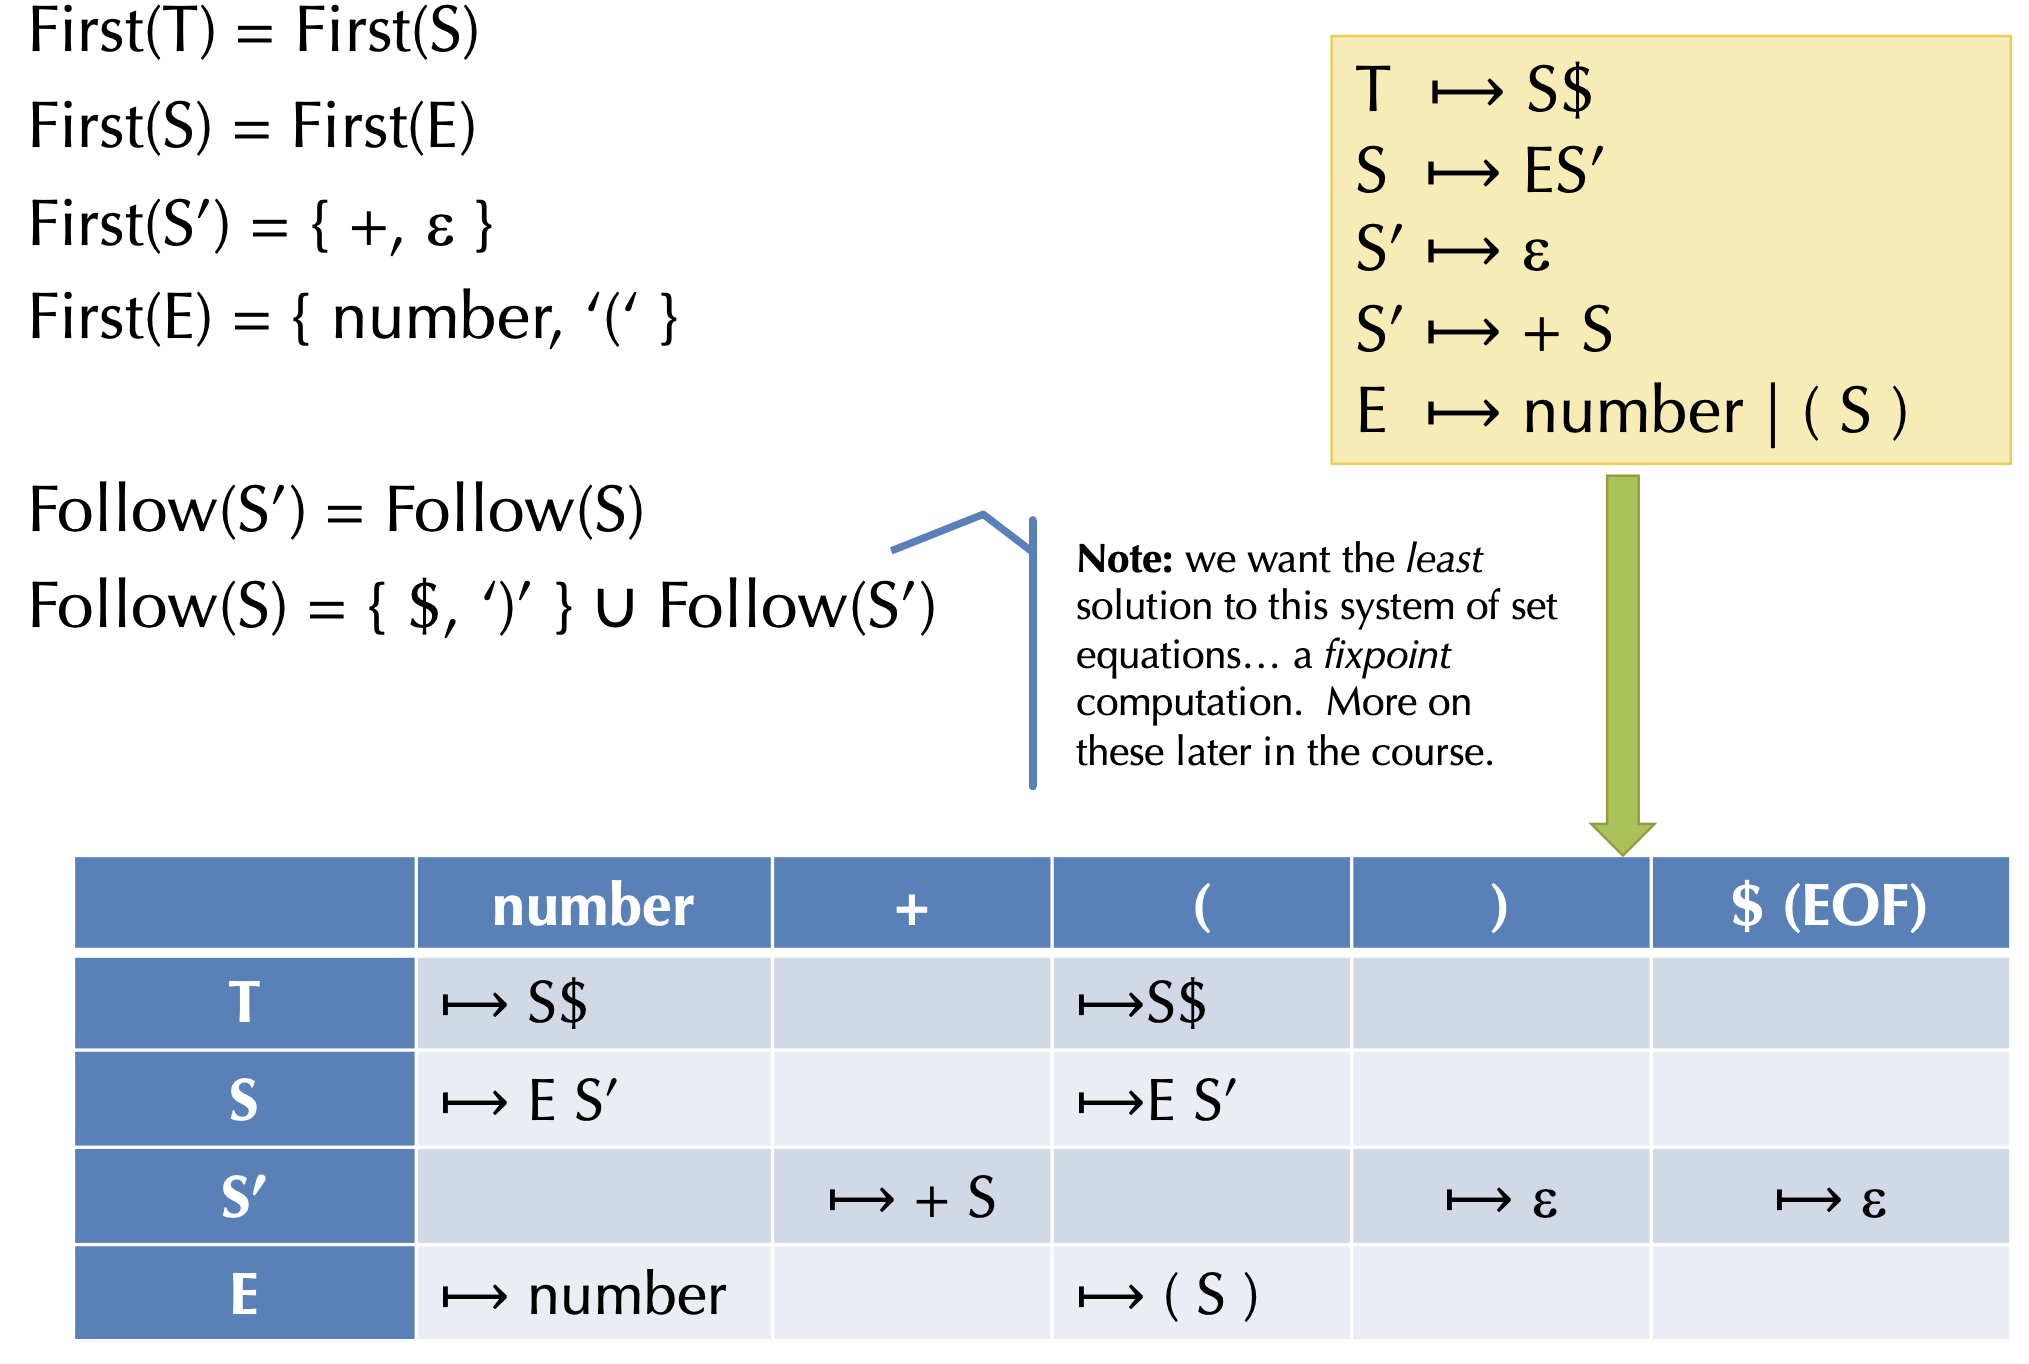
\includegraphics[width=\linewidth]{assets/ll1.png}
\end{center}
\vspace{-10pt}
Intuitively, if we're at nonterminal (\texttt{T, S, S'}) then what productions allow us to parse the terminal (\texttt{+, \$}).

This can be extended to LL($k$) grammars by generating a bigger table.

\textbf{Is it an LL(1) grammar?} No, if there's a cell with multiple options.

\subsection*{LR Grammars and Bottom-Up Parsing}

LR grammars are more expressive than LL grammars. They can handle left-recursive and right-recursive grammars. However error reporting is poorer. \medskip

Bottom-up parsing is a sequence of \textbf{shift} and \textbf{reduce} operations:
\begin{compactitem}
	\item Shift: Move look-ahead token to stack.

	\item Reduce: Replace symbols $\gamma$ at the top of the stack with nonterminal $X$ such that $X \to \gamma$ is a production. Pop $\gamma$, push $X$.
\end{compactitem}

The parser state is made up of a stack of nonterminals and terminals, as well as the so far unconsumed input.\medskip

Action Selection Problem:
\begin{compactitem}
	\item Given a stack $\sigma$ and a lookahead symbol $b$, should the parser \textbf{shift} $b$ onto the stack (new stack is $\sigma b$) , or \textbf{reduce} a production $X \mapsto \gamma$, assuming that $\sigma = \alpha \gamma$?

	\item Sometimes the parser can reduce, but should not, sometimes the stack can be reduced in different ways.
\end{compactitem}

We want to decide based on a prefix $\alpha$ of the stack and the look-ahead. \medskip

In LR(0) we have states: items to track progress on possible upcoming reductions. An item is a production with an extra separator "." in the RHS. \medskip

The idea is that the stuff before the "." is already on the stack and the rest is what might be seen next. \medskip

Constructing the DFA:
\begin{compactitem}
	\item Add new production: $S' \to S\$$, this is the start of the DFA.

	\item Add all productions whose LHS occurs in an item in the state just after the dot. Note that these items can cause more items to be added until a fixpoint is reached (duplicates allowed).

	\item Add transitions for each possible next (non-)terminal. Shift the dot by one in each of those states.

	\item Every state that ends in a dot is a reduce state.
\end{compactitem}
\vspace{-10pt}
\begin{center}
	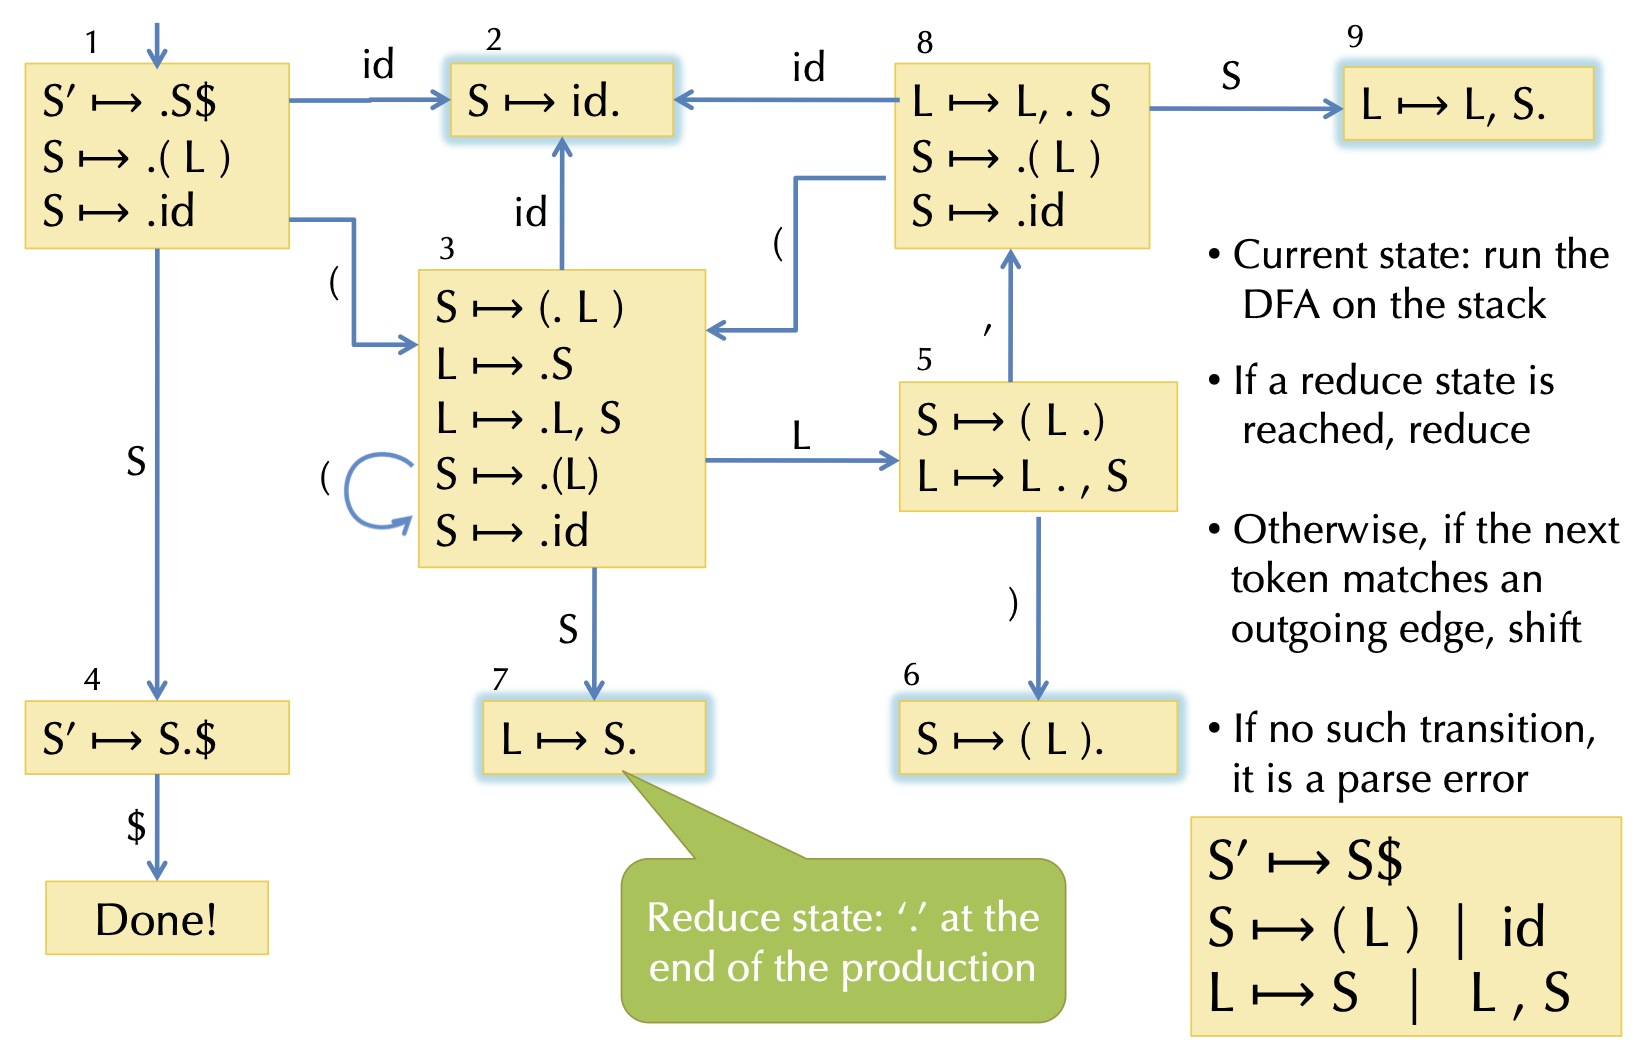
\includegraphics[width=0.8\linewidth]{assets/dfa.png}
\end{center}
\vspace{-10pt}

Instead of running the DFA from start for each step, we can store the state with each symbol on the stack - representing the DFA as a table of shape \texttt{state} $\times$ (\texttt{terminals} + \texttt{nonterminals}). \medskip

An LR(0) machine only works if states with reduce actions have a single reduce action else we will encounter shift/reduce or reduce/reduce conflicts (use LR(1) grammar). \medskip

In LR(1), each item is an LR(0) item plus a set of look-ahead symbols $A \to \alpha . \beta, \; \mathcal L$.\medskip

To form the LR(1) closure, we first do the same as for LR(0). Additionally for each item $C \to . \gamma$ we add due to a rule $A \to \beta . C \gamma, \; \mathcal L$, we compute its look-ahead set $\mathcal M$ including FIRST($\gamma$) and if $\gamma$ can derive $\epsilon$ also $\mathcal L$. \medskip

\vspace{-15pt}
\begin{center}
	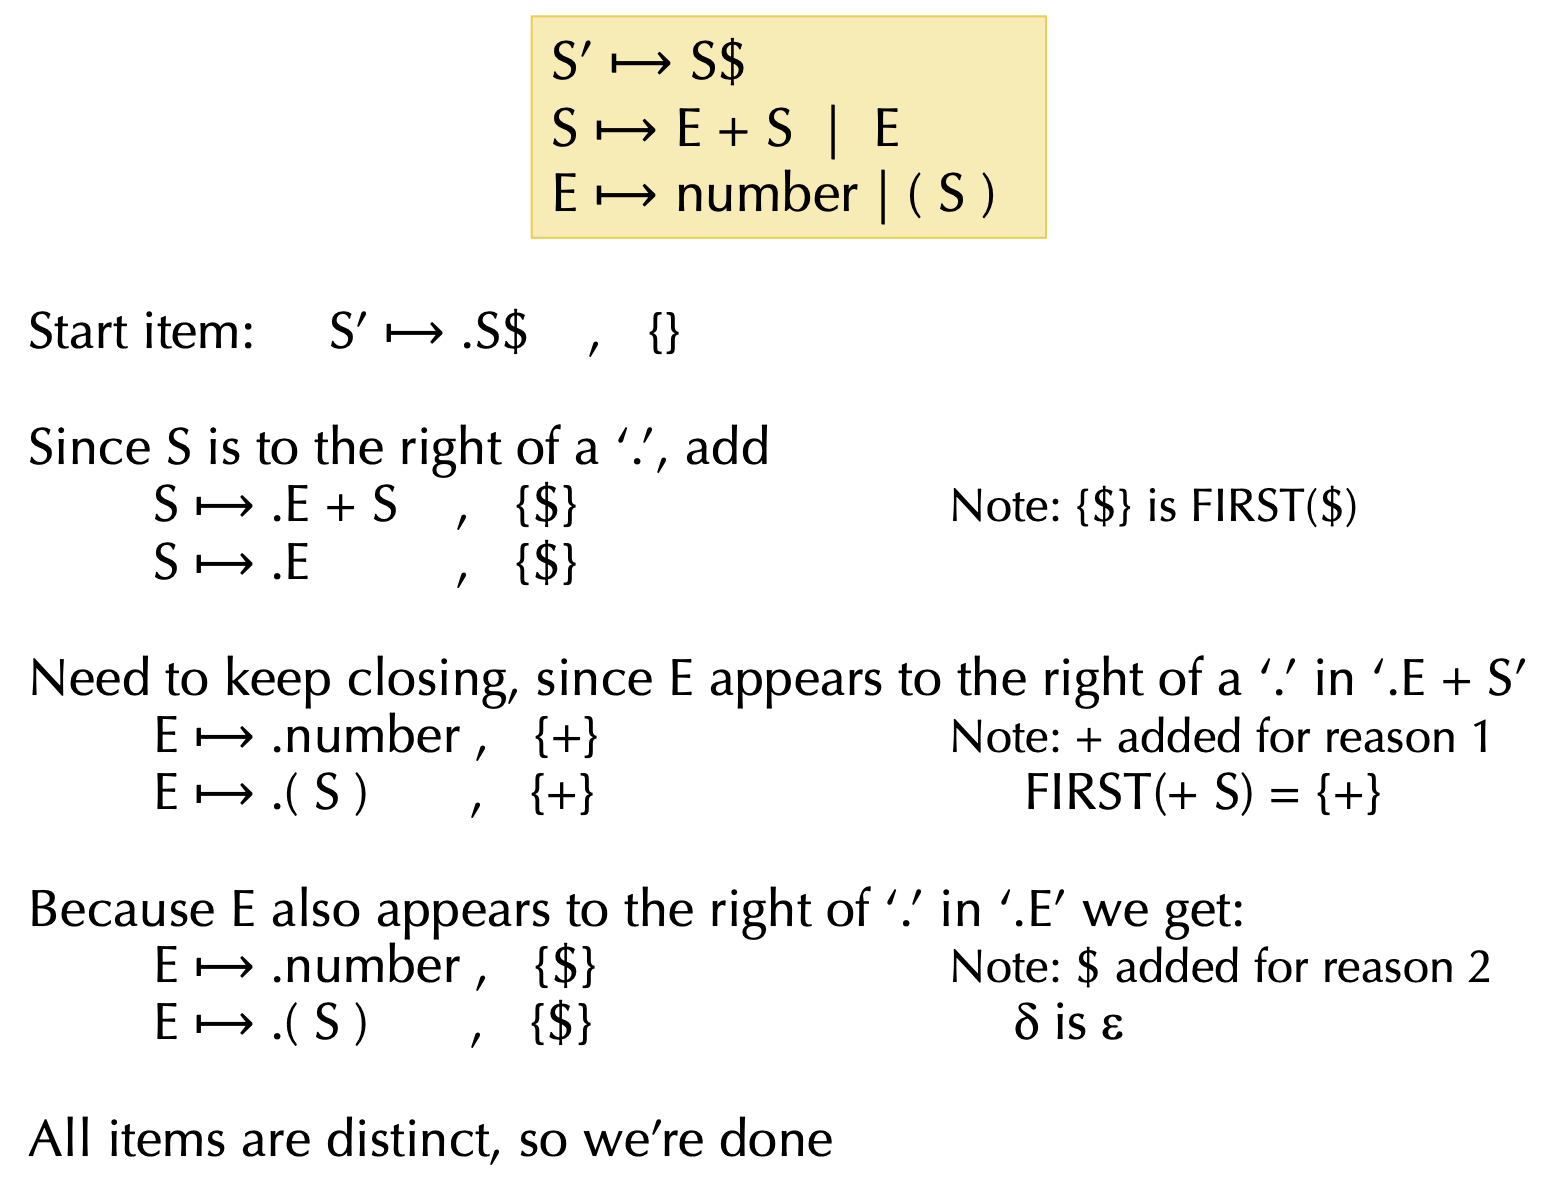
\includegraphics[width=0.8\linewidth]{assets/lr1.png}
\end{center}
\vspace{-10pt}
For LR(1) we have a shift-reduce conflict if the shifted token is contained in the follow set of the reduction.

\begin{multicols*}{2}
	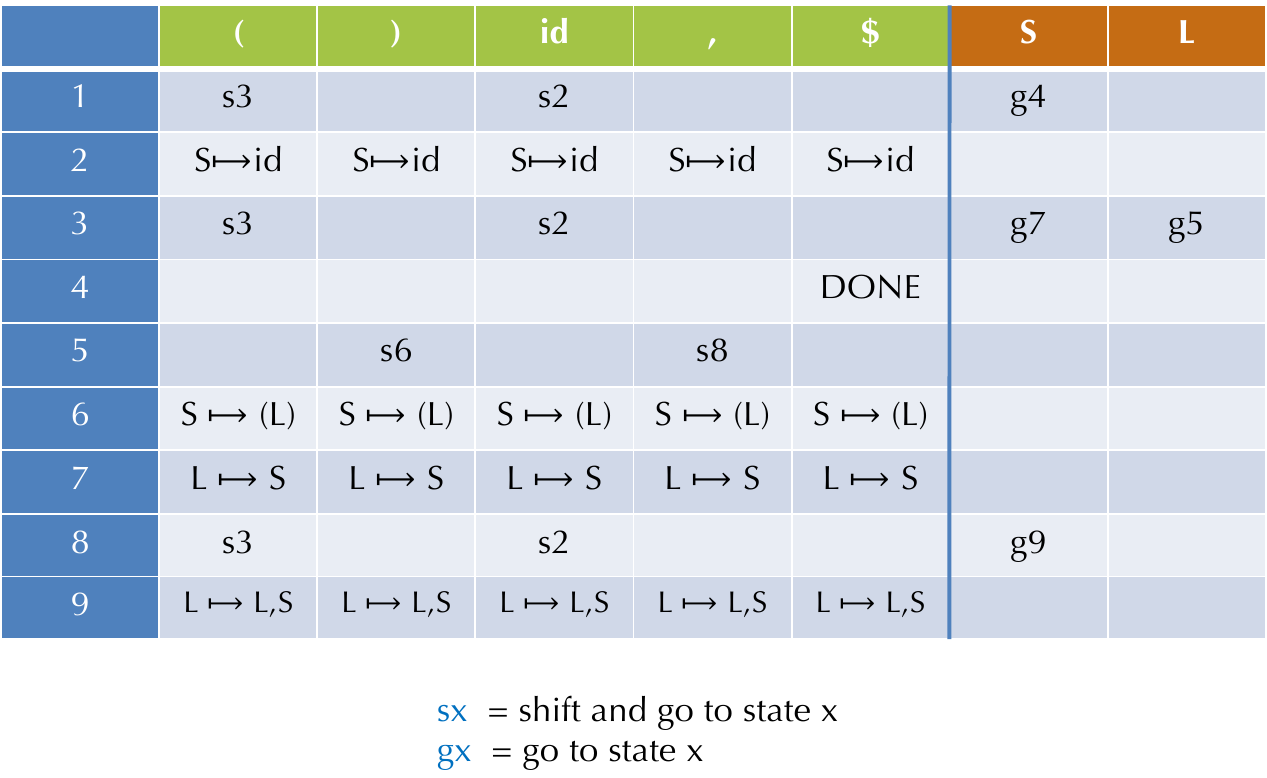
\includegraphics[width=1.15\linewidth]{actiondfa.png}
	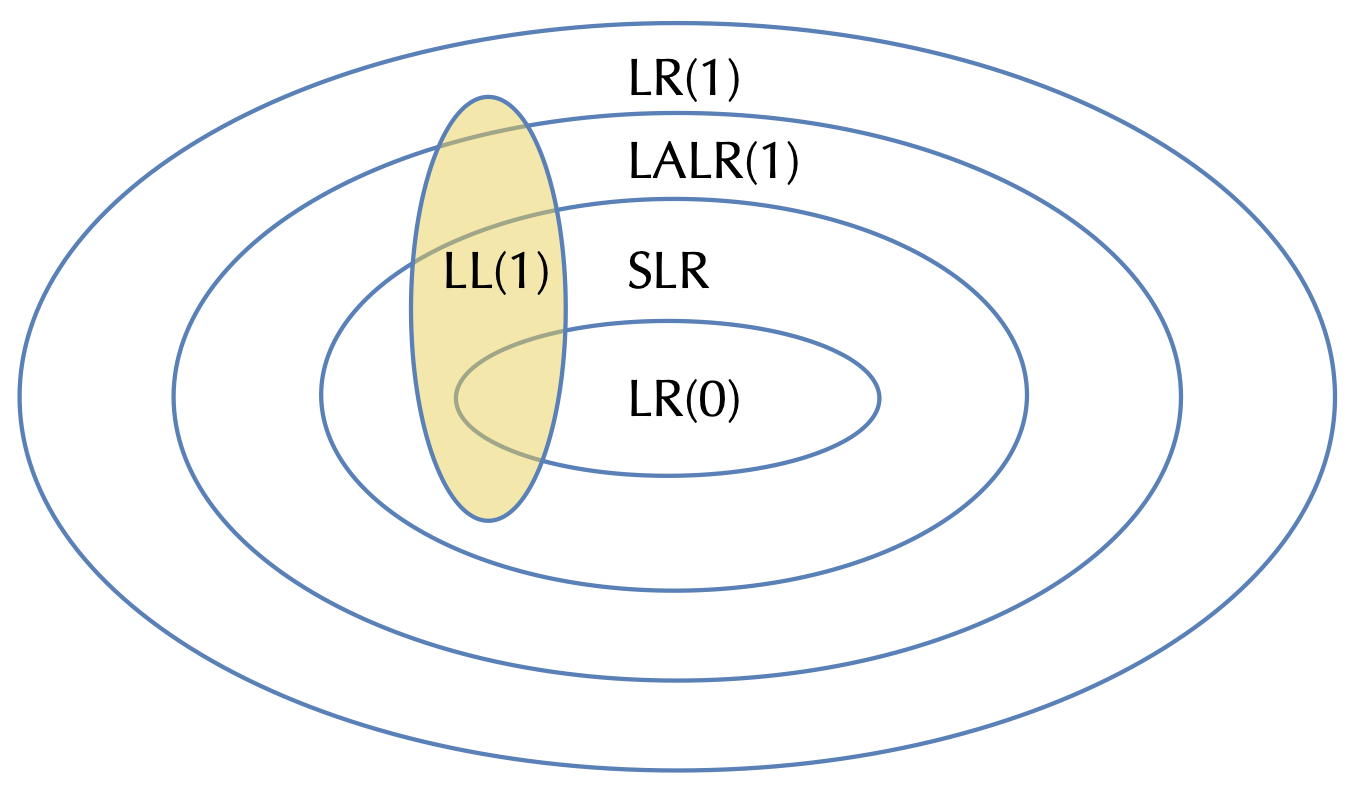
\includegraphics[width=\linewidth]{language.png}
\end{multicols*}
